\PassOptionsToPackage{dvipsnames}{xcolor}
\documentclass{beamer}

\mode<presentation> {

\usetheme{Montpellier} % good one
\usecolortheme{beaver}

%\setbeamertemplate{footline} % To remove the footer line in all slides uncomment this line
\setbeamertemplate{footline}[page number] % To replace the footer line in all slides with a simple slide count uncomment this line

\setbeamertemplate{navigation symbols}{} % To remove the navigation symbols from the bottom of all slides uncomment this line
}

\setbeamertemplate{caption}[numbered]
\setbeamerfont{caption}{size=\scriptsize}
%\usepackage{etex}
\usepackage{array} 
\usepackage{graphicx} % Allows including images
\usepackage{booktabs} % Allows the use of \toprule, \midrule and \bottomrule in tables
\usefonttheme{professionalfonts}
\usepackage{mathptmx}
\usepackage{caption}
\usepackage{subcaption}
\usepackage{amsmath,amsthm,amssymb}
\usepackage{float}
% ------------------ My own stuff
\usepackage[utf8]{inputenc}
\usepackage[T1]{fontenc}

\usepackage{amsmath,amsthm,amssymb}
\DeclareMathOperator*{\argmax}{\arg\!\max}
\DeclareMathOperator*{\argmin}{\arg\!\min}
\DeclareMathOperator{\E}{\mathbb{E}}
\DeclareMathOperator{\R}{\mathbb{R}}

\beamertemplatenavigationsymbolsempty

\usepackage{rotating}
\usepackage{tikz}
\usepackage{fancyvrb}
\usepackage{listings}
\usepackage{verbatim}

%------------------
%	TITLE PAGE
%------------------

\title[CALTeC for CI]{CALTeC : \\ Content-Adaptive Linear Tensor Completion
\\ for \\ Collaborative Intelligence}
\subtitle{ICIP 2021} % The short title appears at the bottom of every slide, the full title is only on the title page

\author[Hans]{ Ashiv Hans Dhondea, Robert A. Cohen and Ivan V. {Bajić}}% Your name
\institute[SFU-Multimedia Lab] 
{
Multimedia Lab\\School of Engineering Science\\Simon Fraser University \\ % Your institution for the title page
\medskip
\centering

\includegraphics[scale=0.5]{SFUhorizontallogorgb.pdf}
}

\date{\today} % Date, can be changed to a custom date

\begin{document}

\begin{frame}
\titlepage % Print the title page as the first slide
\end{frame}

\begin{frame}
\frametitle{Overview} % Table of contents slide, comment this block out to remove it
\tableofcontents % Throughout your presentation, if you choose to use \section{} and \subsection{} commands, these will automatically be printed on this slide as an overview of your presentation
\end{frame}

\section{Collaborative Intelligence}
\begin{frame}
	\frametitle{Introduction: Collaborative Intelligence}
\hl{insert a figure illustrating the principle behind collaborative intelligence.}
\end{frame}

\begin{frame}
	\frametitle{A deep feature tensor}
	\begin{figure}[H]
		\centering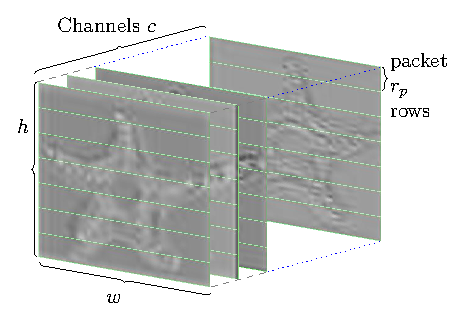
\includegraphics[scale=0.9]{tensorlostviz3icip.pdf}
		\caption{Tensor from layer add\_1 of ResNet-18. Several consecutive rows in each channel form a feature data packet.}
	\end{figure}
\end{frame}

\begin{frame}
	\frametitle{Corrupted tensor visualization}
	\begin{figure}
		\begin{minipage}{.48\textwidth}
			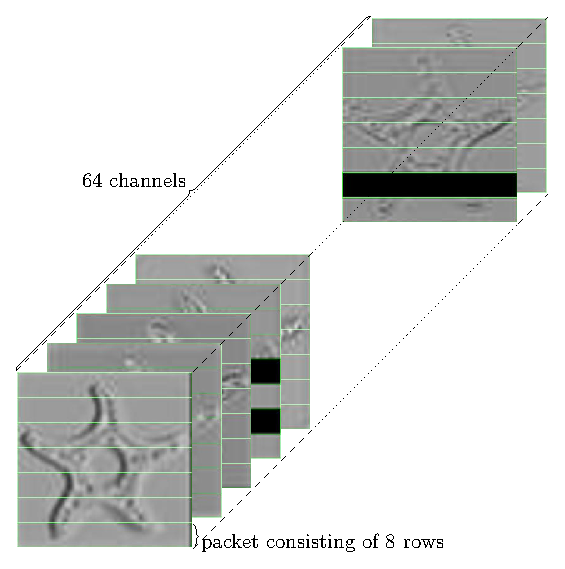
\includegraphics[width=\linewidth]{tensorviz4.pdf}
			\caption{Corrupted ResNet-18 deep feature tensor consisting of 64 channels. Each channel consists of 7 packets. Packets are $8 \times 56$ blocks of deep feature tensor values.}
		\end{minipage}\hfill
		\begin{minipage}{.48\textwidth}
			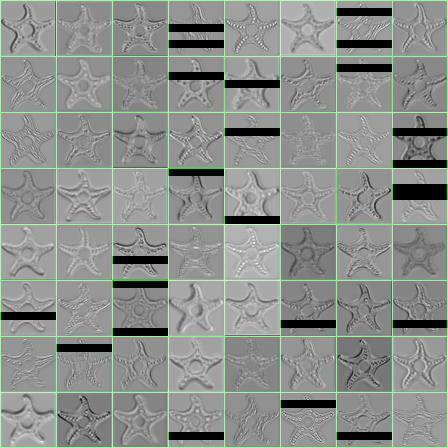
\includegraphics[width=\linewidth]{tiledgridtensor.jpg}
			\caption{Tiled tensor $\tilde{\mathcal{X}} \in \mathbb{R}^{56 \times 56 \times 64}$ visualization. Each tile represents a channel of shape $56 \times 56$. }
		\end{minipage}
	\end{figure}
\end{frame}
%-----------------------------------------------
\end{document} 